
\documentclass[aspectratio=169]{beamer}
%\usetheme{Boadilla}
\usetheme{Warsaw}


\usepackage{listings}
\usepackage{xcolor}
 
\definecolor{codegreen}{rgb}{0,0.6,0}
\definecolor{codegray}{rgb}{0.5,0.5,0.5}
\definecolor{codepurple}{rgb}{0.58,0,0.82}
\definecolor{backcolour}{rgb}{0.95,0.95,0.92}
 
\lstdefinestyle{mystyle}{
    language=Python,
    backgroundcolor=\color{backcolour},   
    commentstyle=\color{codegreen},
    keywordstyle=\color{magenta},
    numberstyle=\tiny\color{codegray},
    stringstyle=\color{codepurple},
    basicstyle=\ttfamily\tiny,
    breakatwhitespace=false,         
    breaklines=true,                 
    captionpos=b,                    
    keepspaces=true,                 
    numbers=left,                    
    numbersep=5pt,                  
    showspaces=false,                
    showstringspaces=false,
    showtabs=false,                  
    tabsize=2
}


\hypersetup{
	colorlinks=true,
	linkcolor=blue,
	urlcolor=cyan
}

 
\lstset{style=mystyle}
%\usepackage{minted}


\usepackage{datetime}
\newdateformat{specialdate}{\twodigit{\THEDAY}-\twodigit{\THEMONTH}-\THEYEAR}
\date{\specialdate\today}


%\renewrobustcmd{\mkbibfootnote}{\normalsize\footnotemark\footnotetext}
\setbeamerfont{footnote}{size=\tiny}

\setbeamertemplate{footline}[frame number]{} % Evita que \pause 
\setbeamertemplate{bibliography item}{\insertbiblabel} % Numeros en las referenicas en vez de iconos




%%%%%%%%%%%%%%%%%%%%%%%%%%%%%%%%%%%%%%%%%%%%%%%%%%%%%%%%%%%%%%%%%%%%%%%%%%%%%
% HEADER
%%%%%%%%%%%%%%%%%%%%%%%%%%%%%%%%%%%%%%%%%%%%%%%%%%%%%%%%%%%%%%%%%%%%%%%%%%%%%

%\title[\arabic{page} ]{Advanced Computer Graphics}
\title[Arrays]{SEARCHING AND SORTING ALGORITHMS}
% Sin subtitulos
\subtitle{6.0001 LECTURE 12}
\author{Kevin Alejandro Hernandez Campillo}
\institute[UPV]{Polytechnic University of Victoria}
\date[]{September-December 2022}
\logo{\pgfimage[width=1cm,height=1cm]{graphics/logo_upv_transparente}}			% Logo on all slides (pdf,png,jpg,eps)
\titlegraphic{
\includegraphics[height=1.5cm]{graphics/logo_upv_transparente} \hfil 
\includegraphics[height=1.5cm]{graphics/python.png}}	% Logo on title slide


\usepackage{etoolbox}
\makeatletter
\patchcmd{\@verbatim}
  {\verbatim@font}
  {\verbatim@font\tiny}
  {}{}
\makeatother


\begin{document}

% Diapositiva de título
\begin{frame}[plain]
  \titlepage
\end{frame}

\begin{frame}[fragile]{SEARCH ALGORITHMS}

\begin{itemize}
\item search algorithm – method for finding an item or group of items with specific properties within a collection of items

\item collection could be implicit
\begin{itemize}
\item example – find square root as a search problem
\begin{itemize}
\item exhaustive enumeration
\item bisection serch
\item Newton-Raphson
\end{itemize}
\end{itemize}
\item collection could be explicit
\begin{itemize}
\item example - is a stident record in a stored collection of data?
\end{itemize}

\end{itemize}
\end{frame}

\begin{frame}[fragile]{SERCHING ALGORITHMS}
\begin{itemize}
\item linear search
\begin{itemize}
\item  \textcolor{red}{brute force} search (aka British Museum algorithm)
\item list does not have to be sorted
\end{itemize}
\item bisection search
\begin{itemize}
\item list \textcolor{red}{MUST be sorted} to give correct answer
\item saw two different implementations of the algorithm
\end{itemize}
\end{itemize}
\end{frame}


\begin{frame}[fragile]{LINEAR SERCH ON \textcolor{red}{UNSORTED} LIST:RECAP}
\begin{lstlisting}
	def linear_serch(L,e):
		found = False
		for i in range(len(L)):
			if e==L[i]:
				found = True
		return found    
\end{lstlisting}
 
\begin{itemize}
\item must look through all elements to decide it’s not there
\item O(len(L)) for the loop*O(1) to test if e == L[i]
\item overall complexity is O(n)-where n is len(L). Assumes we can retrieve element of list in constant time
\item speed up a little by returning True here, but speed up doesn't impact worst case
\begin{lstlisting}
if e==L[i]:
	found = True
\end{lstlisting} 
\end{itemize}
\end{frame}

\begin{frame}[fragile]{LINEAR SERCH ON \textcolor{red}{UNSORTED} LIST:RECAP}
\begin{columns}
\column{0.55\linewidth}
Example code:
\begin{lstlisting}
def linear_serch(L,e):
		found = False
		for i in range(len(L)):
			if e==L[i]:
				found = True
		return found
lista = [4,2,6,7]
print(linear_serch(lista,8))
print(linear_serch(lista,6))
\end{lstlisting}
\column{0.40\linewidth}
Output:
\begin{block}{}
\begin{verbatim}
False
True
\end{verbatim}
\end{block}
\end{columns}
\end{frame}


\begin{frame}[fragile]{LINEAR SERCH ON \textcolor{red}{SORTED} LIST:RECAP}
\begin{lstlisting}
def search(L,e):
	for i in range(len(L)):
		return True
	if L[i] > e:
		return False
	return False
\end{lstlisting}
\begin{itemize}
\item musto only look until reach a number geater than e
\item O(len(L)) for the loop*O(1) to test if e==L[i]
\item overall complexity is \textcolor{red}{O(n)-where n is len(L)}
\end{itemize}
\end{frame}

\begin{frame}[fragile]{LINEAR SERCH ON \textcolor{red}{SORTED} LIST:RECAP}
\begin{columns}
\column{0.55\linewidth}
Example code:
\begin{lstlisting}
def search(L,e):
	for i in range(len(L)):
		return True
	if L[i] > e:
		return False
	return False
lista = [3,4,6,8,9]
print(linear_serch(lista,6))
print(linear_serch(lista,5))
\end{lstlisting}
\column{0.40\linewidth}
Output:
\begin{block}{}
\begin{verbatim}
True
False
\end{verbatim}
\end{block}
\end{columns}
\end{frame}

\begin{frame}{USE BISECTION SERCH: RECAP}
\begin{enumerate}
\item Pick an index, i, that divides list in half
\item Ask if L[i]==e
\item if not, ask if L[i] is larger or smaller than e
\item Depending on answare, sherch left or right half of L for e
\end{enumerate}

A new version of a divide-and conqer algorithm
\begin{itemize}
\item Breake into smaller version of problema(smaller list), puls some simple operations
\item Answare to smaller version is answer to original problem
\end{itemize}
\end{frame}

\begin{frame}{BISECTION SERCH IMPLEMENTATION: RECAP}
\lstinputlisting{bisect_serch2.py}
\end{frame}


\begin{frame}{COMPLEXITY OF BISECTION SEARCH: RECAP}
\begin{itemize}
\item \textcolor{red}{\textbf{bisect\_serch2}} and its helper
\begin{itemize}
\item O(log n) bisection serch calls
\begin{itemize}
\item reduce size of problem by factor of 2 on each step
\end{itemize}
\item pass list and indices as parameters
\item list never copied, just re-passed as pointer
\item constant work inside funcion
\item $\rightarrow$ \textcolor{red}{\textbf{O(log n)}}
\end{itemize}

\end{itemize}

\end{frame}

\begin{frame}[fragile]{BISECTION SERCH IMPLEMENTATION: RECAP}
\begin{columns}
\column{0.65\linewidth}
Example code:
\lstinputlisting{bisect_serch2_ex.py}
\column{0.30\linewidth}
Output:
\begin{block}{}
\begin{verbatim}
True
False
\end{verbatim}
\end{block}
\end{columns}

\end{frame}


\begin{frame}{SEARCHING A SORTED LIST --n is len(L)}
\begin{itemize}
\item using \textcolor{red}{\textbf{linear search}}, search for an element is \textcolor{red}{\textbf{O(n)}}
\item using \textcolor{red}{\textbf{binary search}}, can search for an element in \textcolor{red}{\textbf{O(log n)}}
\begin{itemize}
\item assumes the \textcolor{red}{\textbf{list is sorted!}}
\end{itemize}

\item when does it make sense to \textcolor{red}{\textbf{sort first then search}}?
\begin{itemize}
\item  SORT + O(log n) $<$ O(n) $\rightarrow$ SORT $<$ O(n) - O(log n)
\item when sorAng is less than O(n)
\end{itemize}
\item \textcolor{red}{NEVER TRUE!}
\begin{itemize}
\item to sort a collecEon of n elements must look at each one at
least once!
\end{itemize}
\end{itemize}
\end{frame}

\begin{frame}{AMORTIZED COST --n is len(L)}
\begin{itemize}
\item why bother sorting first?
\item in some cases, may \textcolor{red}{\textbf{sort a list once}} then do \textcolor{red}{\textbf{many searches}}
\item \textcolor{red}{\textbf{AMORTIZE cost}} of the sort over many searches
\item SORT + k\*O(log n) $<$ k\*O(n) \\
	$\rightarrow$ for large K, \textcolor{red}{\textbf{SORT time becomes irrelevant,}} if cost of sorting is small enough
\end{itemize}
\end{frame}

\begin{frame}{SORT ALGORITHMS}
\begin{itemize}
\item  Want to efficiently sort a list of entries (typically
numbers)
\item Will see a range of methods, including one that is
quite efficient
\end{itemize}
\end{frame}

\begin{frame}{MONKEY SORT}
\begin{columns}
\column{0.55\linewidth}
\begin{itemize}
\item aka bogosort, stupid sort, slowsort, permutaAon sort, shotgun sort
\item  to sort a deck of cards
\begin{itemize}
\item throw them in the air
\item pick them up
\item are they sorted?
\item repeat if not sorted
\end{itemize}

\end{itemize}
\column{0.40\linewidth}
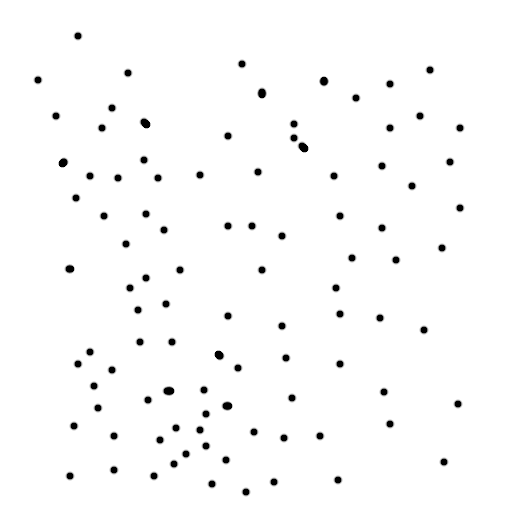
\includegraphics[scale=1]{graphics/monkey_sort.png}
\end{columns}
\end{frame}

\begin{frame}[fragile]{COMPLEXITY OF BOGO SORT}
\begin{lstlisting}
def bogo_sort(L):
	while not is_sorted(L):
		random.shuffle(L)
\end{lstlisting}
\begin{itemize}
\item best case: \textcolor{red}{\textbf{O(n) where n is len(L)}} to check if sorted
\item worst case: O(?) it is \textcolor{red}{\textbf{unbounded}} if really unlucky

\end{itemize}
\end{frame}

\begin{frame}[fragile]{COMPLEXITY OF BOGO SORT}
\begin{columns}
\column{0.65\linewidth}
Example code:
\lstinputlisting{bogo_sort_ex.py}
\column{0.30\linewidth}
Output:
\begin{block}{}
\begin{verbatim}
[1, 2, 7, 9, 10]
\end{verbatim}
\end{block}
\end{columns}

\end{frame}

\begin{frame}{BUBBLE SORT}
\begin{columns}
\column{0.45\linewidth}
\begin{itemize}
\item \textcolor{red}{\textbf{compare consecutive pairs}} of elements
\item \textcolor{red}{\textbf{swap elements}} in pair such that smaller is first
\item when reach end of list,\textcolor{red}{\textbf{start over}} again
\item stop when \textcolor{red}{\textbf{no more swaps}} have been made
\item largest unsorted element always at end a\_er pass, so at most n passes
\end{itemize}
\column{0.45\linewidth}
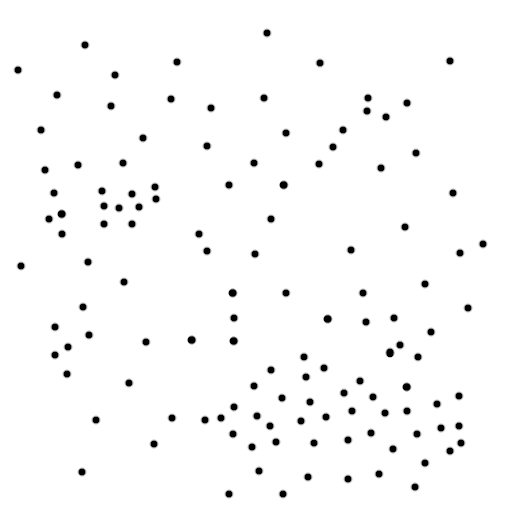
\includegraphics[scale=1]{graphics/bubble_sort.png}
\end{columns}
\end{frame}

\begin{frame}[fragile]{COMPLEXITY OF BUBBLE SORT}
\begin{lstlisting}
def bubble_sort(L):
	swap = False
	while not swap:
		swap = True
		for j in range(1,len(L)):
			if L[j-1] > L[j]:
				swap = False
				temp = L[j]
				L[j] = L[j-1]
				L[j-1] = temp
\end{lstlisting}
\begin{itemize}
\item inner for loop is for doing the \textcolor{red}{\textbf{comparisons}}
\item outer while loop is for doing \textcolor{red}{\textbf{multiple passes}} unti no more swaps
\item \textcolor{red}{\textbf{O($n^2$) where n is len(L)}} to do len(L)\-1 comparsions and len(L)\-1 passes
\end{itemize}
\end{frame}

\begin{frame}[fragile]{COMPLEXITY OF BUBBLE SORT}
\begin{columns}
\column{0.65\linewidth}
Example code:
\begin{lstlisting}
def bubble_sort(L):
    swap = False
    while not swap:
        swap = True
        for j in range(1,len(L)):
            if L[j-1] > L[j]:
                swap = False
                temp = L[j]
                L[j] = L[j-1]
                L[j-1] = temp
    return L    
lista=[7,1,4,5,3]
print(bubble_sort(lista))
\end{lstlisting}
\column{0.30\linewidth}
Output:
\begin{block}{}
\begin{verbatim}
[1, 3, 4, 5, 7]
\end{verbatim}
\end{block}
\end{columns}
\end{frame}

\begin{frame}{SELECTION SORT}
\begin{itemize}
\item first step
\begin{itemize}
\item extract \textcolor{red}{\textbf{minimum element}}
\item \textcolor{red}{\textbf{swap it}} with element at \textcolor{red}{\textbf{index 0}}
\end{itemize}
\item subsequent step
\begin{itemize}
\item in remaining sublist, extract \textcolor{red}{\textbf{minimum element}}
\item \textcolor{red}{\textbf{swap it}} with the element at \textcolor{red}{\textbf{index 1}}
\end{itemize}
\item keep the left portion of the list sorted
\begin{itemize}
\item at i'step, \textcolor{red}{\textbf{first i elements in list are sorted}}
\item all other elements are bigger than first i elements
\end{itemize}
\end{itemize}
\end{frame}


\begin{frame}{ANALYZING SELECTION SORT}
\begin{itemize}
\item loop invariant
\begin{itemize}
\item given prefix of list L[0:i] and suffix L[i+1:len(L)], then prefix is sorted and no element in prefix is larger than smallest element in suffix
\begin{enumerate}
\item  base case: prefix empty, suffix whole list - invariant true
\item  induction step: move minimum element from suffix to end of prefix. Since invariant true before move, prefix sorted after append
\item when exit, prefix is entire list, suffix empty, so sorted
\end{enumerate}
\end{itemize}
\end{itemize}
\end{frame}

\begin{frame}[fragile]{COMPLEXITY OF SELECTION SORT}
\begin{lstlisting}
def selection_sort(L):
	suffixSt = 0
	while suffixSt != len(L):
		for i in range(suffixSt, len(L)):
			if L[i]<L[suffixSt]:
				L[suffixSt], L[i] = L[i], L[suffixSt]
		suffixSt +=1
\end{lstlisting}

\begin{itemize}
\item outer loop executes len(L) times
\item inner loop executes len(L) – i tomes
\item complexity of selection sort is \textcolor{red}{\textbf{O($n2$) where n is len(L)}}
\end{itemize}
\end{frame}

\begin{frame}[fragile]{COMPLEXITY OF SELECTION SORT}
\begin{columns}
\column{0.65\linewidth}
Example code:
\begin{lstlisting}
def selection_sort(L):
    suffixSt = 0
    while suffixSt != len(L):
        for i in range(suffixSt, len(L)):
            if L[i]<L[suffixSt]:
                L[suffixSt], L[i] = L[i], L[suffixSt]
        suffixSt +=1
    return L
lista=[4,2,5,9,3]
print(selection_sort(lista))
\end{lstlisting}
\column{0.30\linewidth}
Output:
\begin{block}{}
\begin{verbatim}
[2, 3, 4, 5, 9]
\end{verbatim}
\end{block}
\end{columns}
\end{frame}

\begin{frame}{MERGE SORT}
\begin{itemize}
\item use a divide-and-conquer approach:
\begin{enumerate}
\item if list is of length 0 or 1, already sorted
\item if list has more than one element, split into two lists, and sort each
\item merge sorted sublists
\begin{enumerate}
\item look at first element of each, move smaller to end of the result
\item when one list empty, just copy rest of other list
\end{enumerate}
\end{enumerate}
\end{itemize}
\end{frame}

\begin{frame}{MERGE SORT}
\begin{itemize}
\item divide and conquer
\end{itemize}
\begin{center}
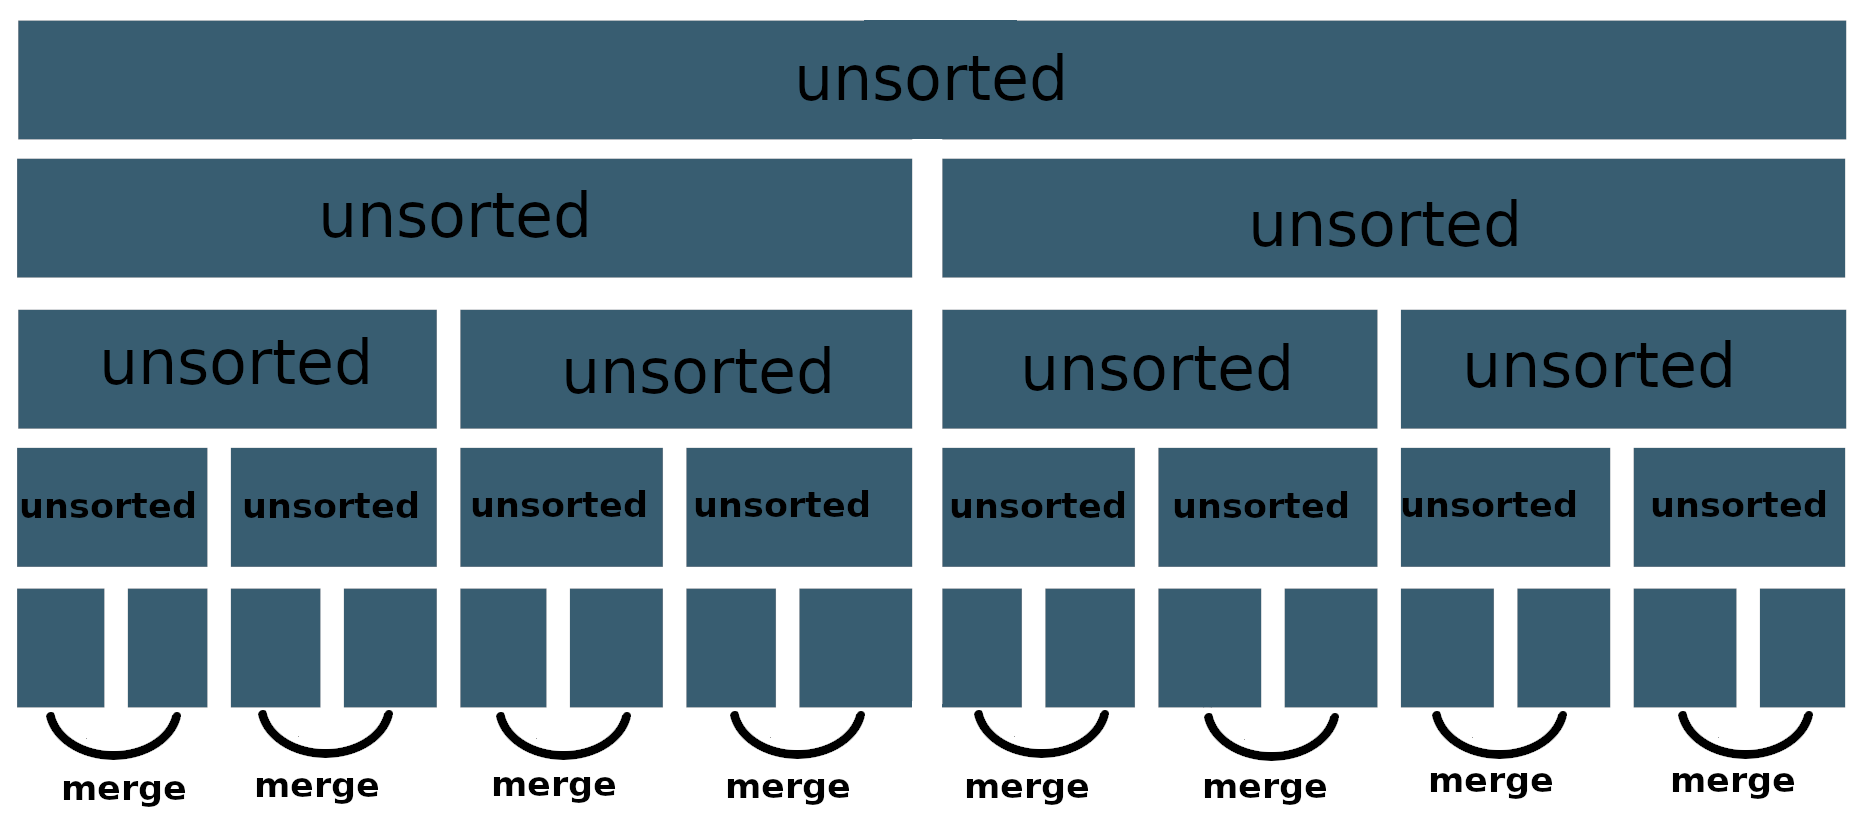
\includegraphics[scale=0.70]{graphics/marge_sort.png}
\end{center}
\begin{itemize}
\item \textcolor{red}{\textbf{split list in half}} until have sublists of only 1 element

\end{itemize}

\end{frame}

\begin{frame}{MERGE SORT}
\begin{itemize}
\item divide and conquer
\end{itemize}
\begin{center}
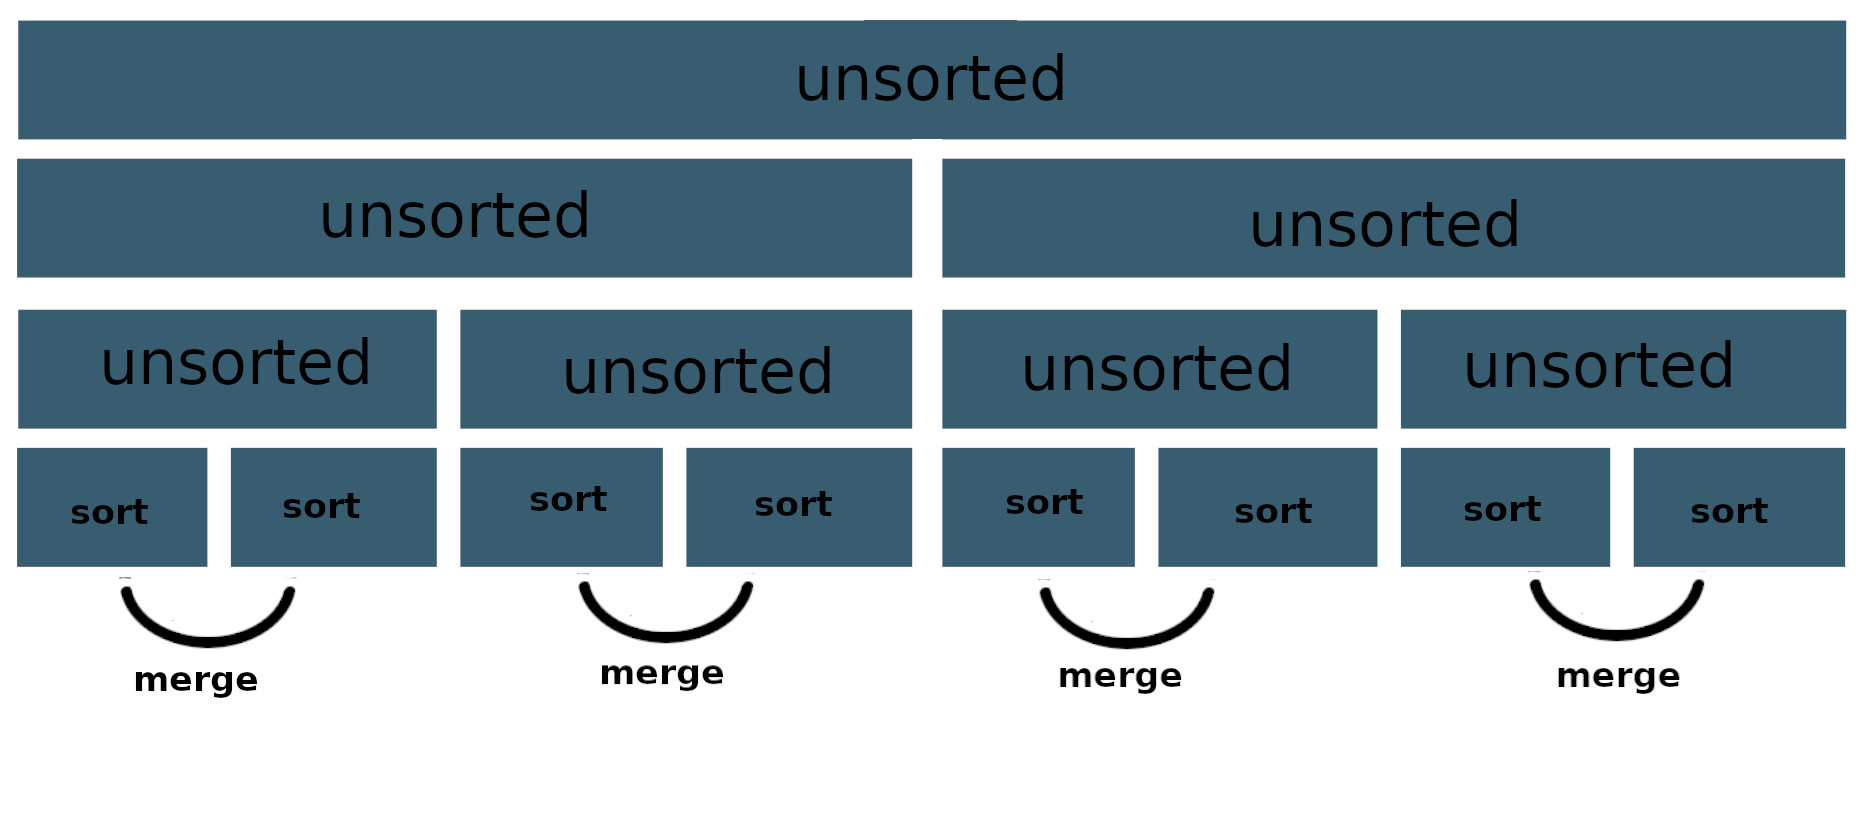
\includegraphics[scale=0.70]{graphics/marge_sort2.png}
\end{center}
\begin{itemize}
\item merge such that \textcolor{red}{\textbf{sublists will be sorted after merge}}
\end{itemize}
\end{frame}

\begin{frame}{MERGE SORT}
\begin{itemize}
\item divide and conquer
\end{itemize}
\begin{center}
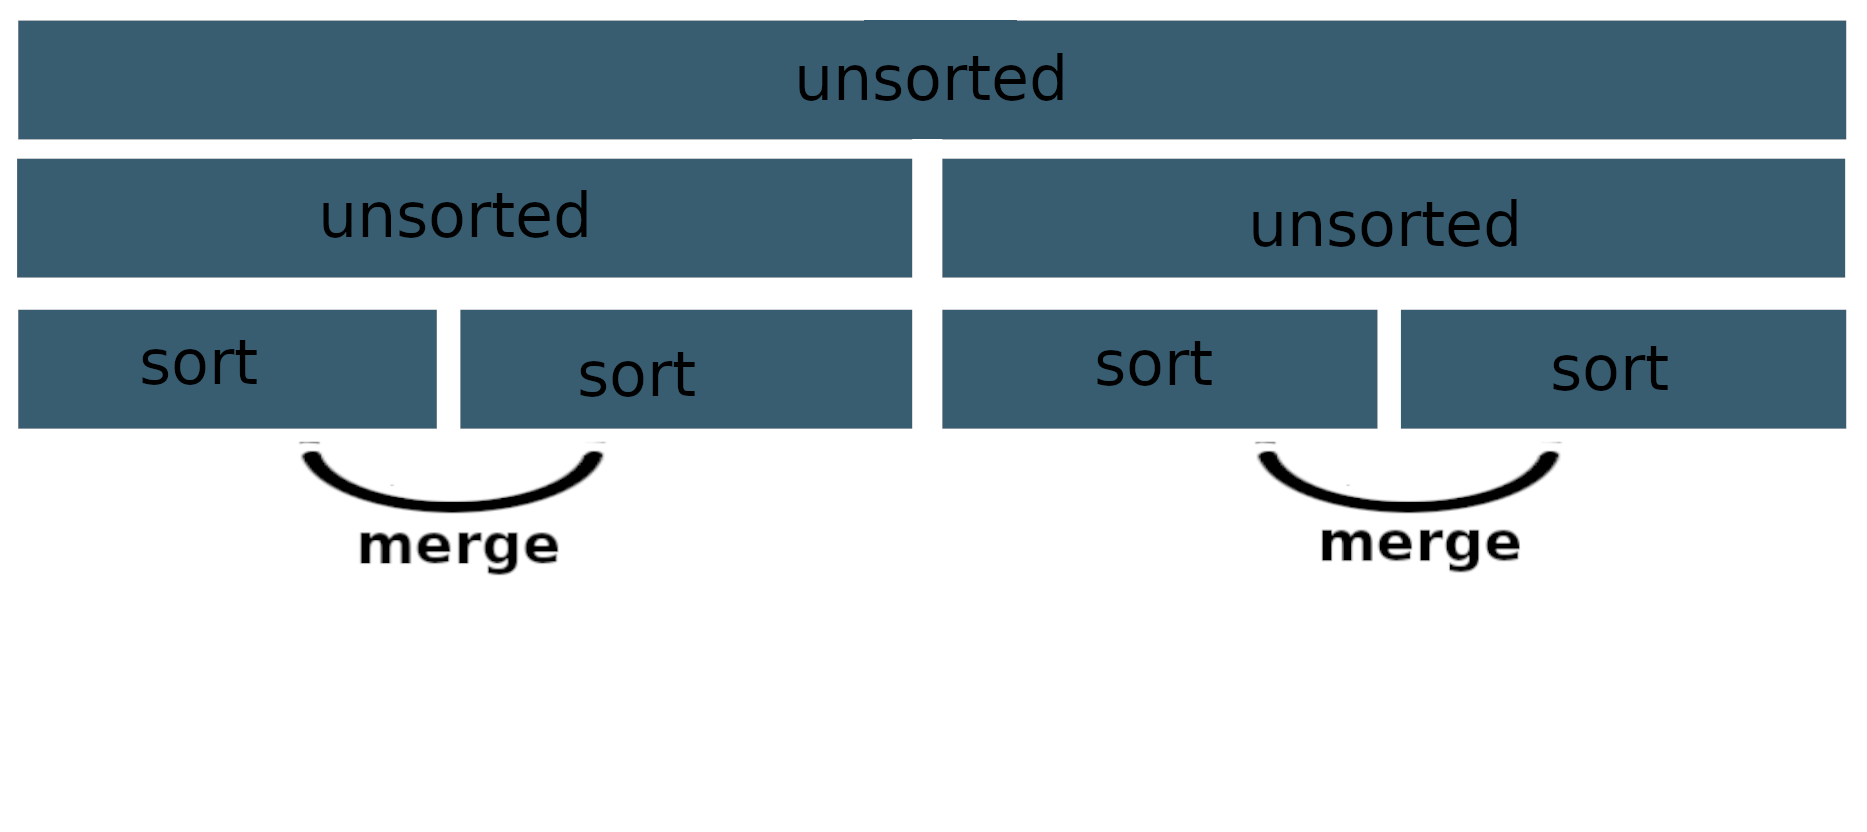
\includegraphics[scale=0.70]{graphics/marge_sort3.png}
\end{center}
\begin{itemize}
\item merge sorted sublists
\item sublists will bee sorted after merge
\end{itemize}
\end{frame}

\begin{frame}{MERGE SORT}
\begin{itemize}
\item divide and conquer
\end{itemize}
\begin{center}
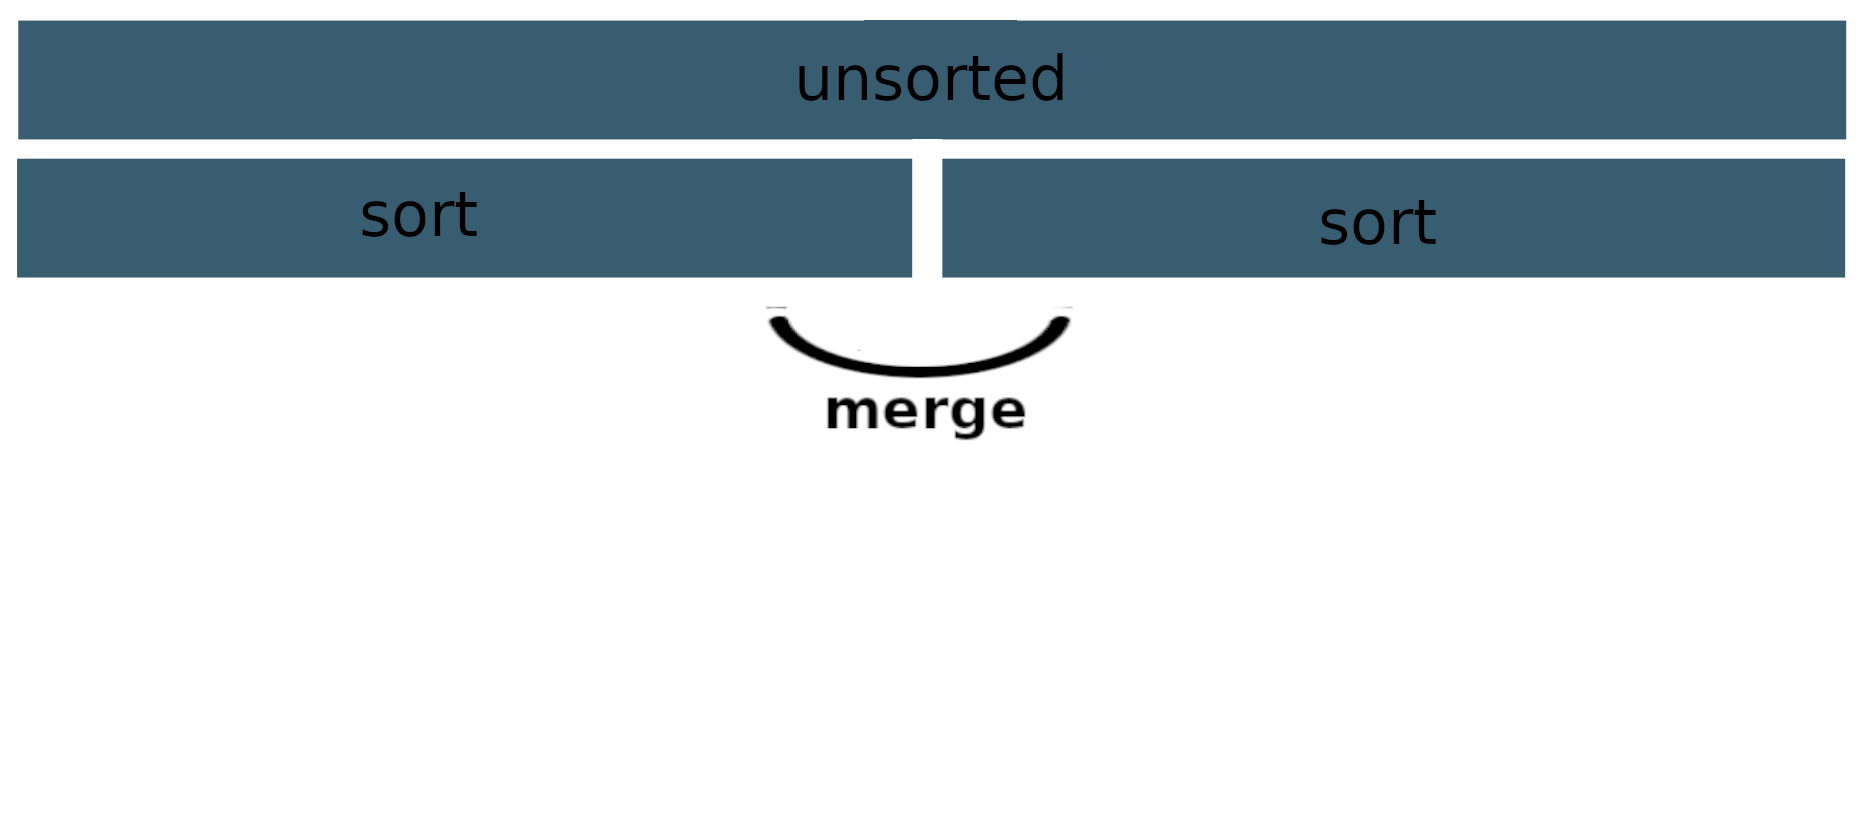
\includegraphics[scale=0.70]{graphics/marge_sort4.png}
\end{center}
\begin{itemize}
\item merge sorted sublists
\item soblists will be sorted after merge
\end{itemize}
\end{frame}

\begin{frame}{MERGE SORT}
\begin{itemize}
\item divide and conquer - done!
\end{itemize}
\begin{center}
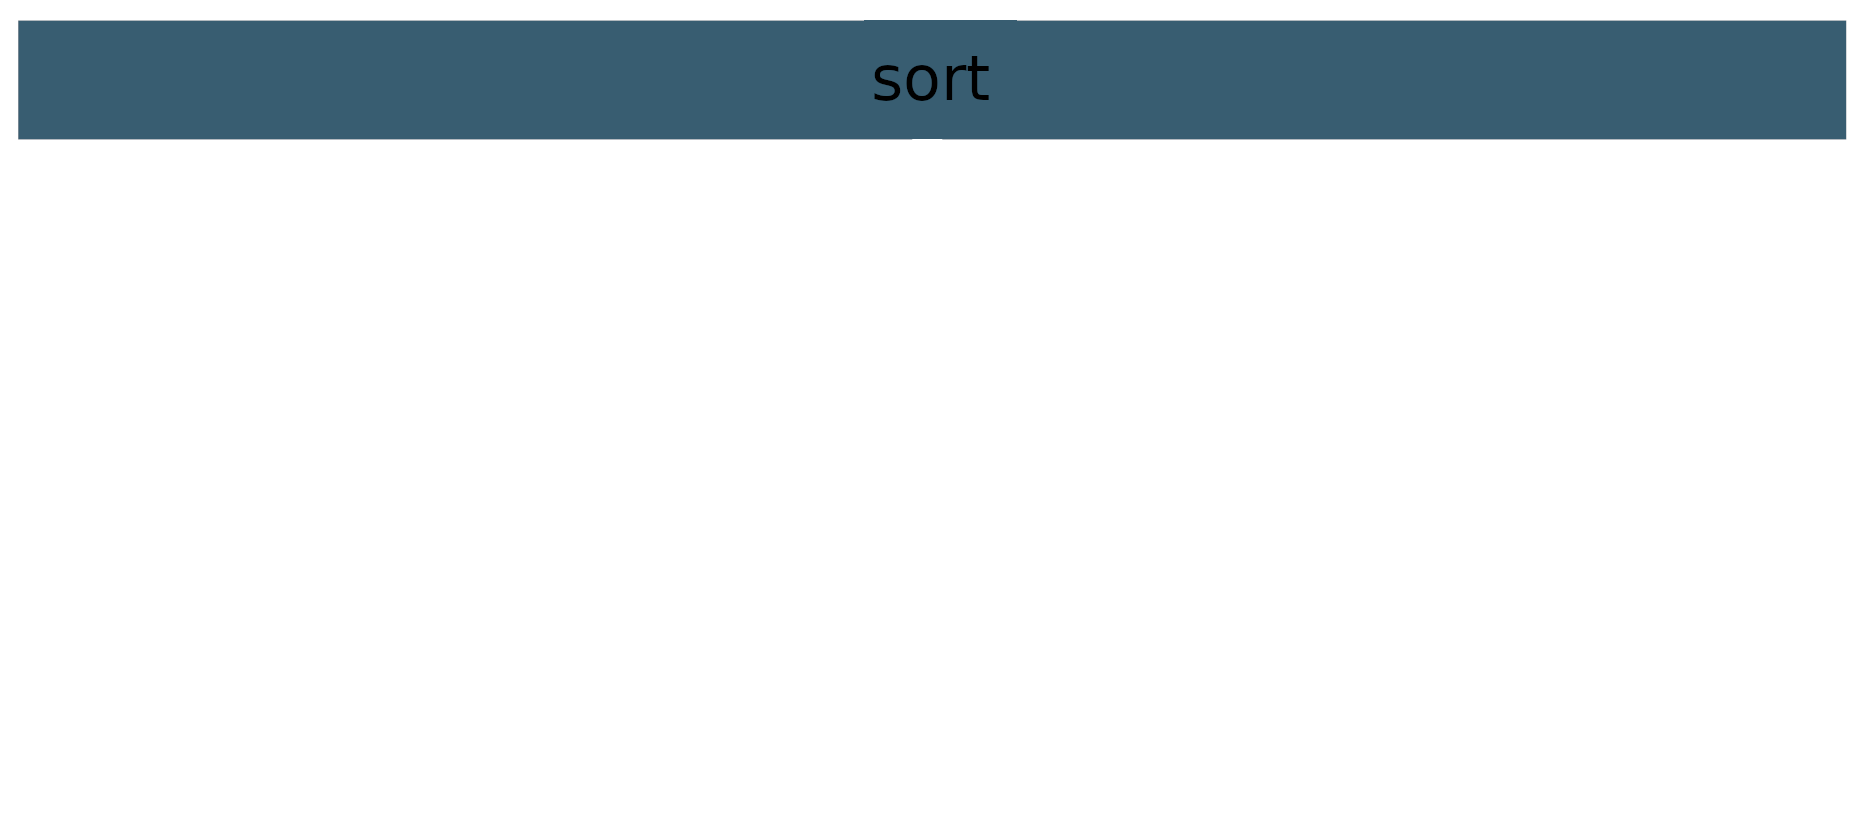
\includegraphics[scale=0.70]{graphics/marge_sort5.png}
\end{center}
\end{frame}

\begin{frame}{EXAMPLE OF MERGING}
\begin{columns}
\column{0.24\linewidth}
Left in list 1\par
[1,5,12,18,19,20]\par
[5,12,18,19,20]\par
[5,12,18,19,20]\par
[5,12,18,19,20]\par
[5,12,18,19,20]\par
[12,18,19,20]\par
[18,19,20]\par
[18,19,20]\par
[]
\column{0.24\linewidth}
Left in list 2\par
[2,3,4,17]\par
[2,3,4,17]\par
[3,4,17]\par
[4,17]\par
[17]\par
[17]\par
[17]\par
[]\par
[]
\column{0.2\linewidth}
Compare\par
1,2\par
5,2\par
5,3\par
5,4\par
5,17\par
12,17\par
18,17\par
18,--
\column{0.28\linewidth}
Result\par
[]\par
[1]\par
[1,2]\par
[1,2,3]\par
[1,2,3,4]\par
[1,2,3,4,5]\par
[1,2,3,4,5,12]\par
[1,2,3,4,5,12,17]\par
[1,2,3,4,5,12,17,18,19,20]
\end{columns}
\end{frame}

\begin{frame}[fragile]{MERGING SUBLISTS STEP}
\begin{lstlisting}
def merge(left, right):
	result = []
	i,j = 0,0
	while i < len(left) and j < len(right):
		if left[i] < right[j]:
			result.append(left[i])
			i += 1
		else:
			result.append(right[j])
			j += 1
	while (i < len(left)):
		result.append(left[i])
		i += 1
	while (j < len(right)):
		result.append(right[j])
		j += 1
	return result

\end{lstlisting}

\end{frame}


\begin{frame}[fragile]{MERGING SUBLISTS STEP - CODE EXPLAINED}
\begin{lstlisting}
if left[i] < right[j]:
	result.append(left[i])
	i += 1
else:
	result.append(right[j])
	j += 1
\end{lstlisting}
\begin{itemize}
\item left and right sublists are ordered
\item move indices for sublists depending on which sublist holds next smallest element
\end{itemize}
\begin{lstlisting}
while (i < len(left)):
		result.append(left[i])
		i += 1
\end{lstlisting}
\begin{itemize}
\item when right sublist is empty
\end{itemize}

\begin{lstlisting}
while (j < len(right)):
		result.append(right[j])
		j += 1
\end{lstlisting}
\begin{itemize}
\item when left sublist is empty
\end{itemize}
\end{frame}

\begin{frame}[fragile]{MERGING SUBLISTS}
\begin{columns}
\column{0.65\linewidth}
Example code:
\begin{lstlisting}
def merge(left, right):
    result = []
    i,j = 0,0
    while i < len(left) and j < len(right):
        if left[i] < right[j]:
            result.append(left[i])
            i += 1
        else:
            result.append(right[j])
            j += 1
    while (i < len(left)):
        result.append(left[i])
        i += 1
    while (j < len(right)):
        result.append(right[j])
        j += 1
    return result
lista1=[2,4,7,9]
lista2=[3,8,13]
merge(lista1,lista2)
\end{lstlisting}
\column{0.40\linewidth}
Output:
\begin{block}{}
\begin{verbatim}
[2, 3, 4, 7, 8, 9, 13]
\end{verbatim}
\end{block}
\end{columns}
\end{frame}

\begin{frame}{COMPLEXITY OFMERGING SUBLISTS STEP}
\begin{itemize}
\item go through two lists, only one pass
\item compare only \textcolor{red}{\textbf{smallest elements in each sublist}}
\item O(len(left) + len(right)) copied elements
\item O(len(longer list)) comparisons
\item \textcolor{red}{\textbf{linear in length of the lists}}
\end{itemize}
\end{frame}

\begin{frame}[fragile]{MERGE SORT ALGORITHM -- RECURSIVE}
\begin{lstlisting}
def merge_sort(L):
	if len(L) < 2:
		return L[:]
	else:
		middle = len(L)//2
		left = merge_sort(L[:middle])
		right = merge_sort(L[middle:])
		return merge(left, right)
\end{lstlisting}
\begin{itemize}
\item \textcolor{red}{\textbf{divide list}} successively into halves
\item depth-first such that \textcolor{red}{\textbf{conquer smallest pieces down one branch}} first before moving to larger pieces
\end{itemize}
\end{frame}

\begin{frame}
\begin{center}
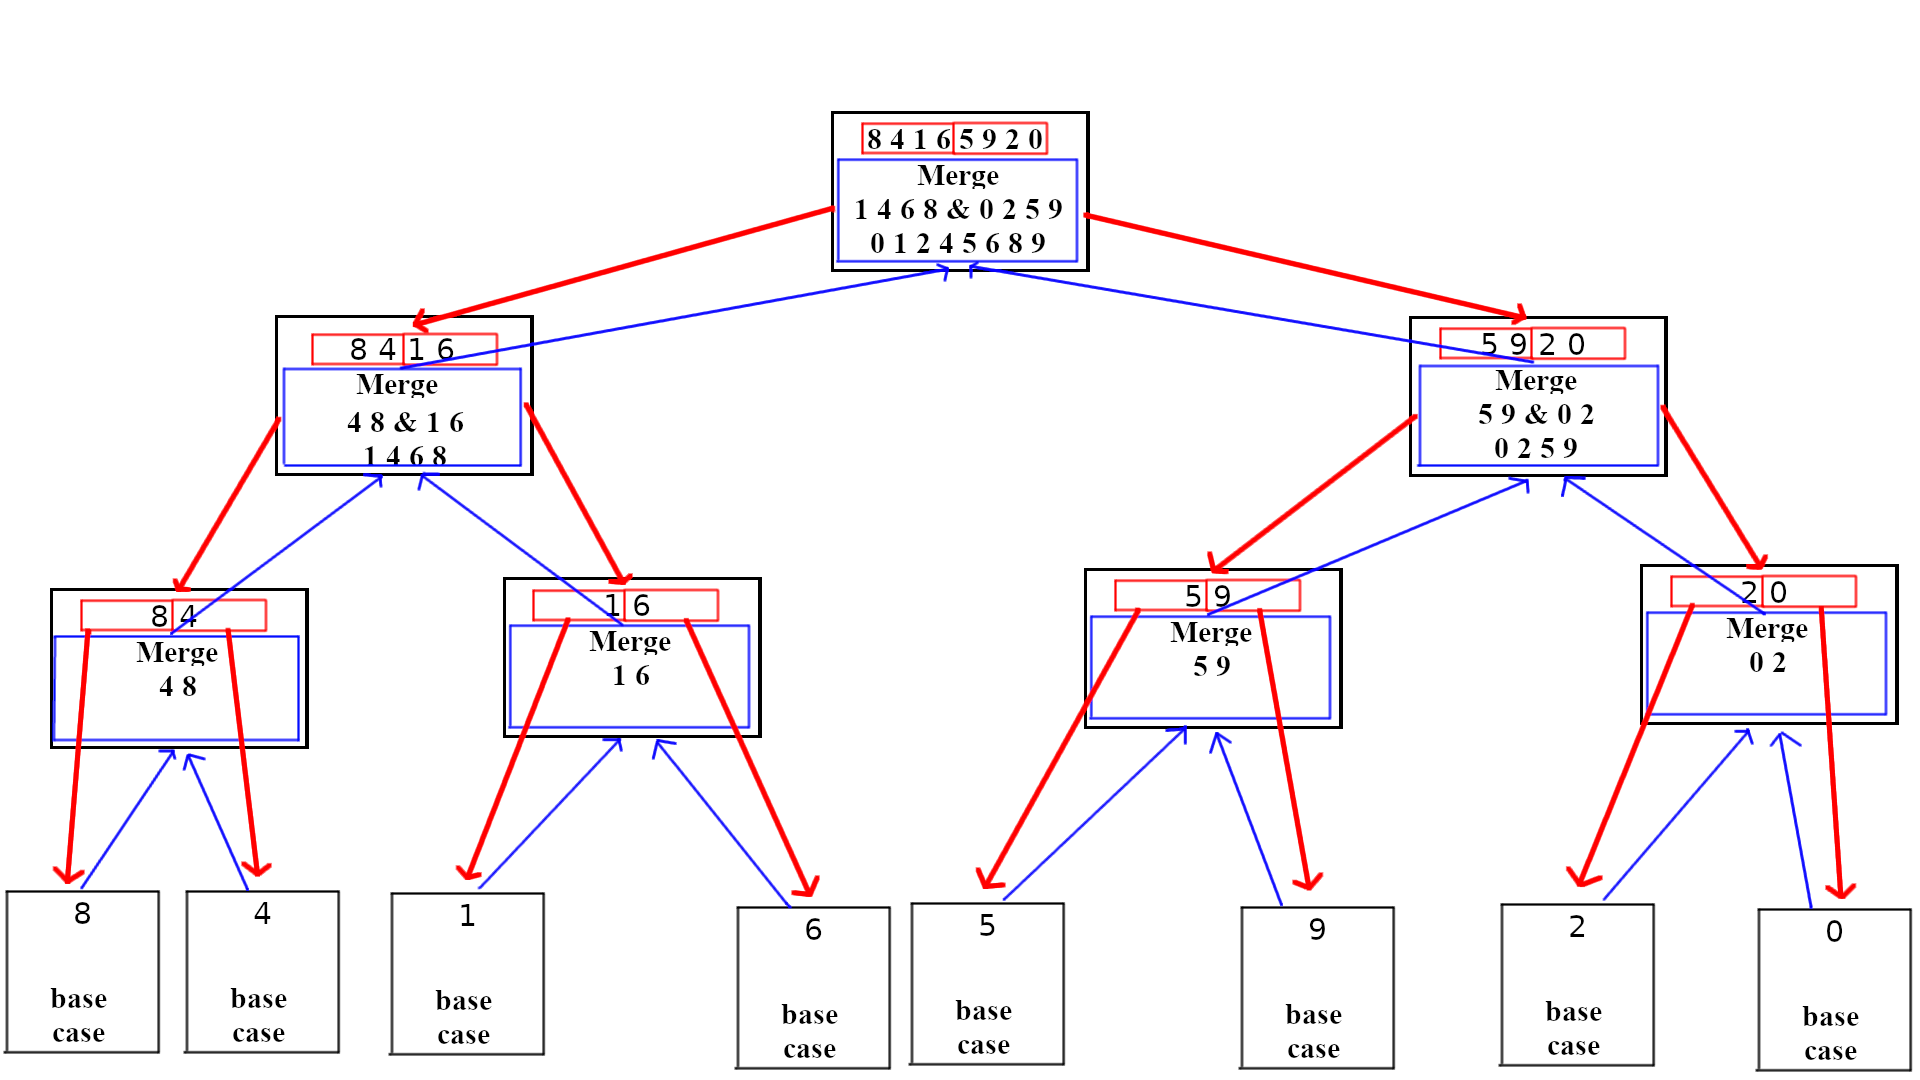
\includegraphics[scale=0.8]{graphics/merge_sort_dia.png}
\end{center}
\end{frame}

\begin{frame}{COMPLEXITY OF MERGE SORT}
\begin{itemize}
\item \textcolor{red}{\textbf{at first recursion level}}
\begin{itemize}
\item n/2 elements in each list
\item O(n) + O(n) = O(n) where n is len(L)
\end{itemize}
\item at \textcolor{red}{\textbf{second recorsion level}}
\begin{itemize}
\item n/4 elements in each list
\item two merges $\rightarrow$ O(n) where n is len(L)
\end{itemize}
\item each recursion level is O(n) where n is len(L)
\item \textcolor{red}{\textbf{dividing list in half}} with each recursive call
\begin{itemize}
\item O(log(n)) where n is len(L)
\end{itemize}
\item overall complexity is \textcolor{red}{\textbf{O(n log(n)) where n is len(L)}}
\end{itemize}
\end{frame}


\begin{frame}{SORTING SUMMARY --n is len(L)}
\begin{itemize}
\item bogo sort
\begin{itemize}
\item randomness, unbonded O()
\end{itemize}
\item bubble sort
\begin{itemize}
\item O($n^2$)
\end{itemize}
\item selection sort
\begin{itemize}
\item O($n^2$)
\item guaranteed the first i elements were sorted
\end{itemize}
\item merge sort
\begin{itemize}
\item O(n log(n))
\end{itemize}
\item O(n log(n)) is the fastest a sort can be
\end{itemize}
\end{frame}

\begin{frame}
\Huge{WHAT HAVE WE SEEN IN 6.0001?}
\end{frame}

\begin{frame}{KEY TOPICS}
\begin{itemize}
\item represent knowledge with \textcolor{red}{\textbf{data structures}}
\item \textcolor{red}{\textbf{iteration and recursion}} as computational metaphors
\item \textcolor{red}{\textbf{abstraction}} of procedures and data types
\item \textcolor{red}{\textbf{organize and modularize}} systems using object classes and methods
\item different classes of \textcolor{red}{\textbf{algorithms}}, searching and sorAng
\item \textcolor{red}{\textbf{complexity}} of algorithms
\end{itemize}
\end{frame}

\begin{frame}{OVERVIEW OF COURSE}
\begin{itemize}
\item learn computational modes of thinking
\item begin to master the art of computational problem solving
\item make computers do what you want them to do
\end{itemize}
Hope we have started you down the path to being able to think and act like a computer scientist
\end{frame}


\begin{frame}{WHAT DO COMPUTER SCIENTISTS DO?}
\begin{columns}
\column{0.50\linewidth}
\begin{itemize}
\item they think computationally
\begin{itemize}
\item abstractions, algorithms, automated execution
\end{itemize}
\item just like the three r’s: reading, ‘riting, and ‘rithmetic -
computational thinking is becoming a fundamental skill that
every well-educated person will need
\end{itemize}


\column{0.40\linewidth}
\begin{columns}
\column{0.23\linewidth}
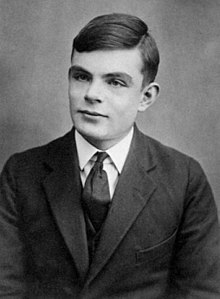
\includegraphics[scale=0.34]{graphics/alan_turing.jpg}
\tiny{Alan Turing
Image in the Public Domain, courtesy of \href{https://es.wikipedia.org/wiki/Alan_Turing}{Wikipedia Commons}.}
\column{0.23\linewidth}
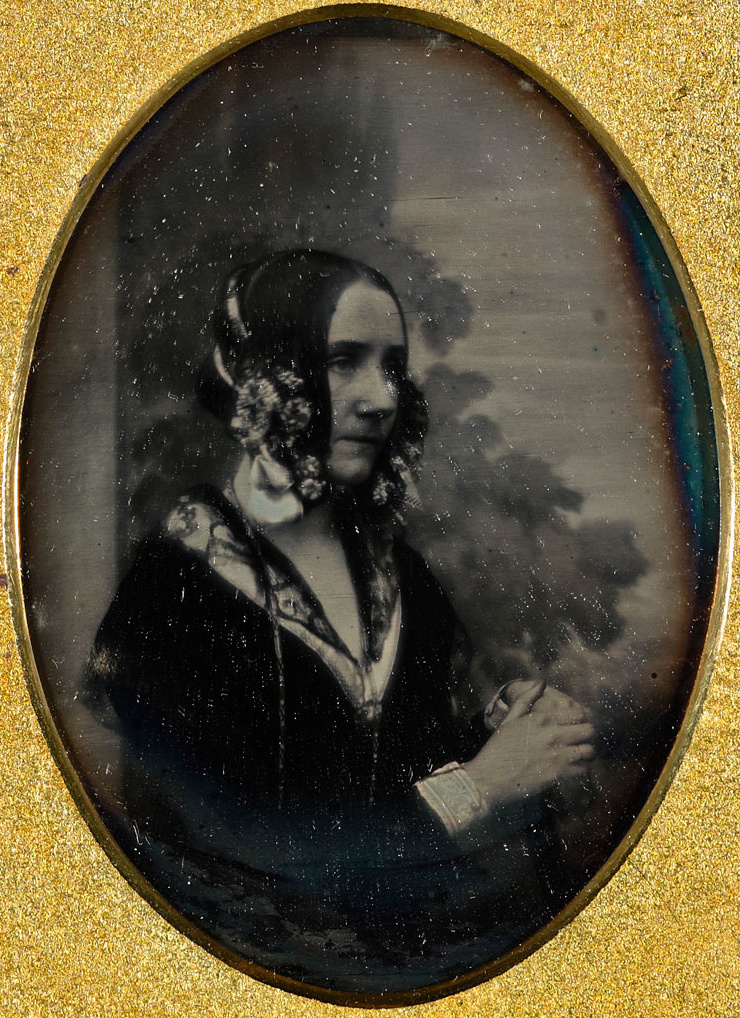
\includegraphics[scale=0.4]{graphics/ada_lovelace.jpg}
\tiny{Ada Lovelace
Image in the Public Domain, courtesy of \href{https://es.wikipedia.org/wiki/Ada_Lovelace}{Wikipedia Commons}.}
\end{columns}
\end{columns}
\end{frame}

\begin{frame}{THE THREE A’S OF COMPUTATIONAL THINKING}
\begin{itemize}
\item abstraction
\begin{itemize}
\item choosing the right abstractions
\item operationg in multiple layers of abstraction simultaneously
\item defining the relationships between the abstraction layers
\end{itemize}
\item automation
\begin{itemize}
\item think in terms of mechanizing our abstractions
\item mechanization is possible – because we have precise and exacting notations and models; and because there is some “machine” that can interpret our notations
\end{itemize}
\item algorithms
\begin{itemize}
\item anguage for describing automated processes
\item also allows abstaction of details
\item language for communicating ideas \& processes
\end{itemize}
\end{itemize}
\end{frame}

\begin{frame}{ASPECTS OF COMPUTATIONAL THINKING}
\begin{itemize}
\item how difficult is this problem and how best can I solve it?
\begin{itemize}
\item theoretical computer science gives precise meaning to these
and related questions and their answers
\end{itemize}
\item thinking recursively
\begin{itemize}
\item reformulating a seemingly difficult problem into onewhich we know how to solve
\item reduction, embedding, transformation, simulaAon

\end{itemize}
\end{itemize}
\end{frame}

\begin{frame}
MIT OpenCourseWare\\
\url{https://ocw.mit.edu}
\par
\vspace{1cm}
6.0001 Introduction to Computer Science and Programming in Python\\
Fall 2016\\
\par
\vspace{2cm}
For information about citing these materials or our Terms of Use, visit:\url{https://ocw.mit.edu/terms}

\end{frame}
\end{document}

